\documentclass[10pt, a4paper]{article}

\usepackage{graphicx}
\usepackage[utf8]{inputenc}
\usepackage{nameref}
\usepackage{listings}             % used for code examples
\usepackage[]{csquotes}
\usepackage{hyperref}
\usepackage[T1]{fontenc}
\usepackage[ngerman]{babel}
\usepackage{subfigure}

\title{Übungsblatt 1}

\author{Sven Fiergolla, 1252732}

\begin{document}
\maketitle

\section*{Aufgabe 1}
\subsection*{1.1}
\begin{itemize}
\item Zustand: Die aktuelle Position aller Scheiben ist der Zustand des Spiels. Beispielsweise ist der Zustand zu Beginn des Spiels, dass alle Scheiben auf Position A liegen.
\item Operator: Das umpositionieren der je obersten Scheibe eines Stapels. Beispielsweise das Verschieben der ersten Scheibe von Stapel A auf Stapel B.
\item Zielbedingung: Alle Scheiben liegen der größe nach geordnet auf Position C.
\item Pfadkosten: Die Anzahl der Züge welche zum Erreichen der Zielbedingung benötigt werden.
\end{itemize}

\subsection*{1.2}
Zustandsmege für 3 Scheiben:\\
$\{\{1,2,3\},\{\},\{\}\}$\\
$\{\{\},\{1,2,3\},\{\}\}$\\\medskip
$\{\{\},\{\},\{1,2,3\}\}$\\ 
$\{\{2,3\},\{1\},\{\}\}$\\
$\{\{2,3\},\{\},\{1\}\}$\\
$\{\{1\},\{2,3\},\{\}\}$\\
$\{\{\},\{2,3\},\{1\}\}$\\
$\{\{1\},\{\},\{2,3\}\}$\\\medskip
$\{\{\},\{1\},\{2,3\}\}$\\
$\{\{1,3\},\{2\},\{\}\}$\\
$\{\{1,3\},\{\},\{2\}\}$\\
$\{\{2\},\{1,3\},\{\}\}$\\
$\{\{\},\{1,3\},\{2\}\}$\\
$\{\{2\},\{\},\{1,3\}\}$\\\medskip
$\{\{\},\{2\},\{1,3\}\}$\\ 
$\{\{3\},\{1\},\{2\}\}$\\
$\{\{3\},\{2\},\{1\}\}$\\
$\{\{2\},\{3\},\{1\}\}$\\
$\{\{2\},\{1\},\{3\}\}$\\
$\{\{1\},\{2\},\{3\}\}$\\
$\{\{1\},\{3\},\{2\}\}$\\

\subsection*{1.3}
Sind $n$ Scheiben vorgegeben, so braucht man mindestens $2^{n-1}$ Schritte.

\section*{Aufgabe 2}
\subsection*{2.1}
Suchraum unklar in Folien definiert!\medskip\\
Köln, Berlin, Trier, München\\
Köln, Berlin, München, Trier\\
Köln, Trier, Berlin, München\\
Köln, Trier, München, Berlin\\
Köln, München, Trier, Berlin\\
Köln, München, Berlin, Trier\\
Trier, Berlin, Köln, München\\
Trier, Berlin, München, Köln\\
Trier, München, Berlin, Köln\\
Trier, München, Köln, Berlin\\
Trier, Köln, München, Berlin\\
Trier, Köln, Berlin, München\\
Berlin, München, Trier, Köln\\
Berlin, München, Köln, Trier\\
Berlin, Trier, München, Köln\\
Berlin, Trier, Köln, München\\
Berlin, Köln, Trier, München\\
Berlin, Köln, München, Trier\\
München, Trier, Köln, Berlin\\
München, Trier, Berlin, Köln\\
München, Köln, Trier, Berlin\\
München, Köln, Berlin, Trier\\
München, Berlin, Köln, Trier\\
München, Berlin, Trier, Köln\\

\subsection*{2.2}
Trier, Berlin, Köln, München = 2409\\
Trier, München, Köln, Berlin = 2409\\
Trier, Berlin, München, Köln = 2092\\
Trier, Köln, München, Berlin = 2092\\
Trier, Köln, Berlin, München = 1891\\
Trier, München, Berlin, Köln = 1891\\

\begin{figure}[htbp]
     \begin{center}
%
        \subfigure{%
            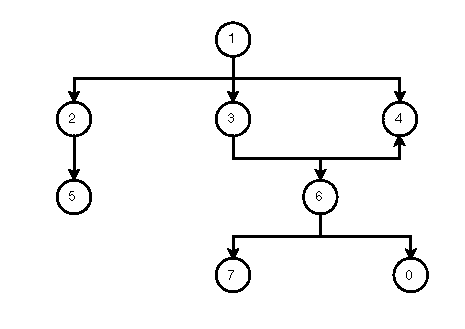
\includegraphics[width=0.4\textwidth]{pdf/breitensuche0.pdf}
        }%
        \subfigure{%
           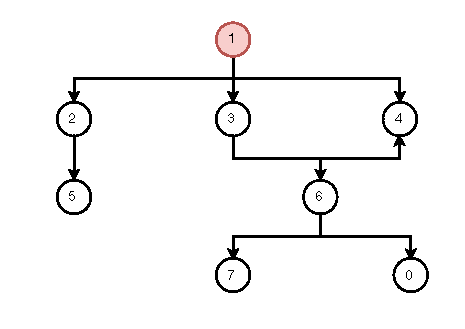
\includegraphics[width=0.4\textwidth]{pdf/breitensuche1.pdf}
        }\\ %  ------- End of the first row ----------------------%
        \subfigure{%
            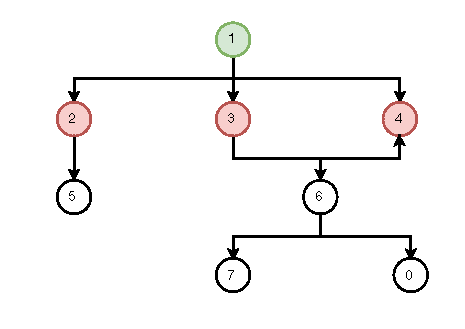
\includegraphics[width=0.4\textwidth]{pdf/breitensuche2.pdf}
        }%
        \subfigure{%
            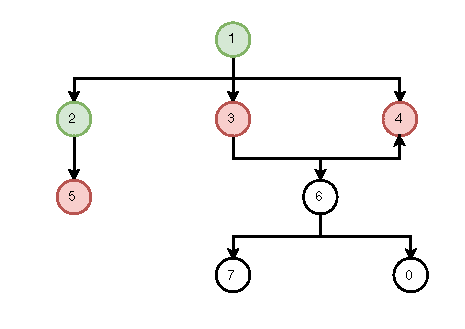
\includegraphics[width=0.4\textwidth]{pdf/breitensuche3.pdf}
        }\\%
        
             \subfigure{%
            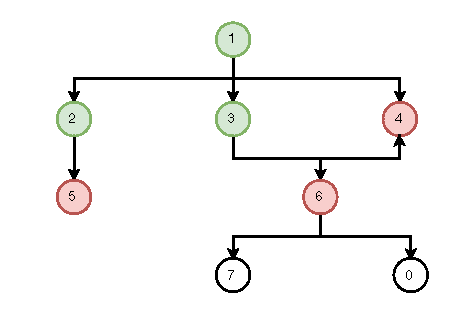
\includegraphics[width=0.4\textwidth]{pdf/breitensuche4.pdf}
        }%
        \subfigure{%
            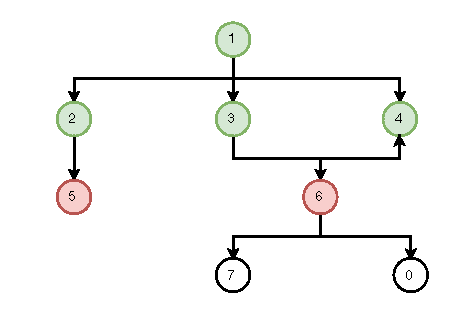
\includegraphics[width=0.4\textwidth]{pdf/breitensuche5.pdf}
        }\\
        
             \subfigure{%
            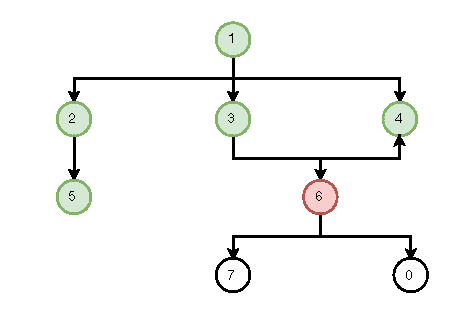
\includegraphics[width=0.4\textwidth]{pdf/breitensuche6.pdf}
        }%
        \subfigure{%
            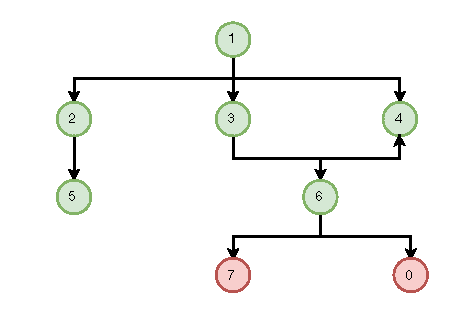
\includegraphics[width=0.4\textwidth]{pdf/breitensuche7.pdf}
        }\\
             \subfigure{
            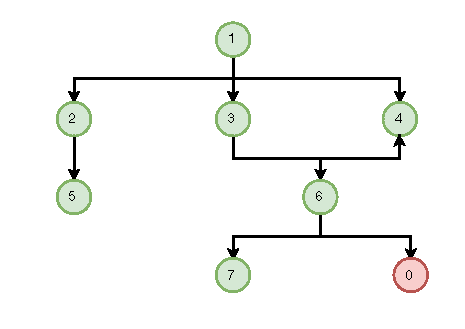
\includegraphics[width=0.4\textwidth]{pdf/breitensuche8.pdf}
        }        \subfigure{
            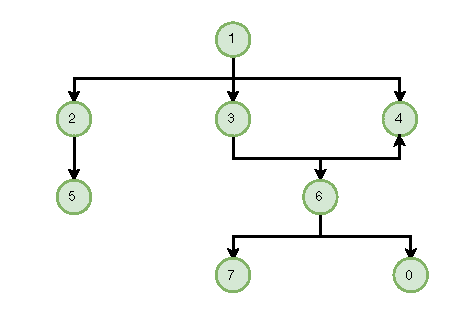
\includegraphics[width=0.4\textwidth]{pdf/breitensuche9.pdf}
        }
   
    \end{center}
    \caption{%
        Breitensuche im Baum. Rot = Knoten in Queue, Grün = Besuchte Knoten
     }%
   \label{fig:subfigures}
\end{figure}

\begin{figure}[htbp]
     \begin{center}
%
        \subfigure{%
            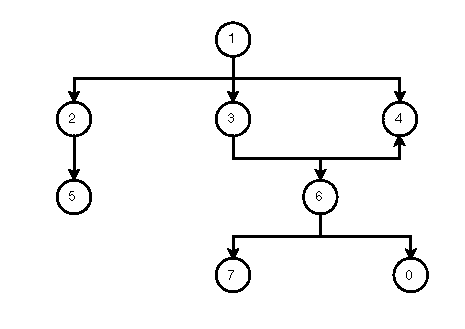
\includegraphics[width=0.4\textwidth]{pdf/tiefensuche0.pdf}
        }%
        \subfigure{%
           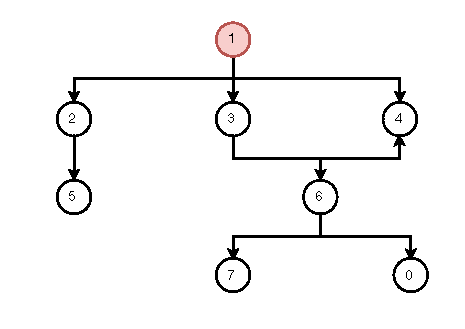
\includegraphics[width=0.4\textwidth]{pdf/tiefensuche1.pdf}
        }\\ %  ------- End of the first row ----------------------%
        \subfigure{%
            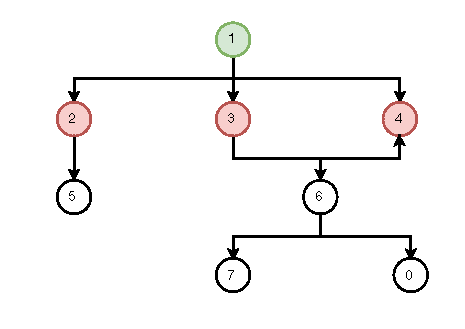
\includegraphics[width=0.4\textwidth]{pdf/tiefensuche2.pdf}
        }%
        \subfigure{%
            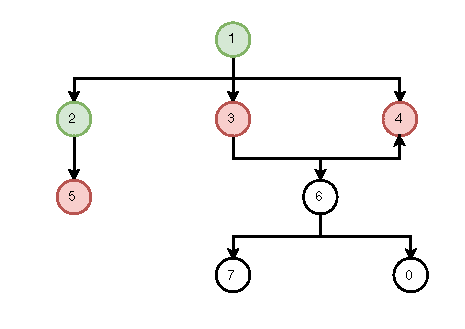
\includegraphics[width=0.4\textwidth]{pdf/tiefensuche3.pdf}
        }\\%
        
             \subfigure{%
            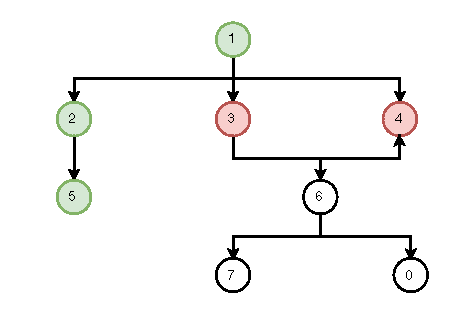
\includegraphics[width=0.4\textwidth]{pdf/tiefensuche4.pdf}
        }%
        \subfigure{%
            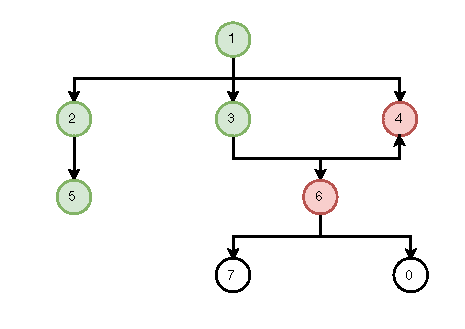
\includegraphics[width=0.4\textwidth]{pdf/tiefensuche5.pdf}
        }\\
        
             \subfigure{%
            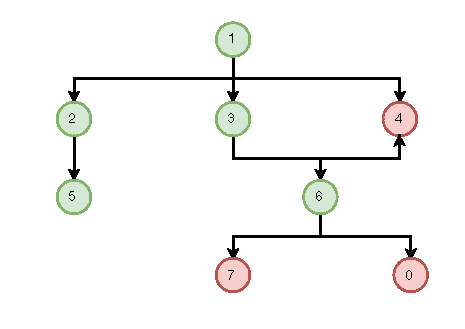
\includegraphics[width=0.4\textwidth]{pdf/tiefensuche6.pdf}
        }%
        \subfigure{%
            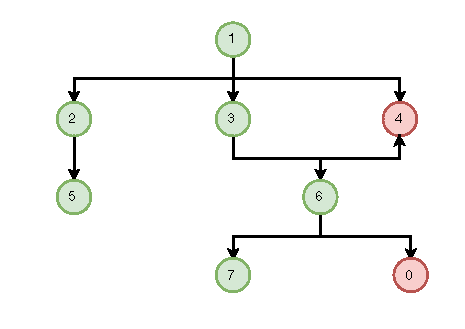
\includegraphics[width=0.4\textwidth]{pdf/tiefensuche7.pdf}
        }\\
             \subfigure{
            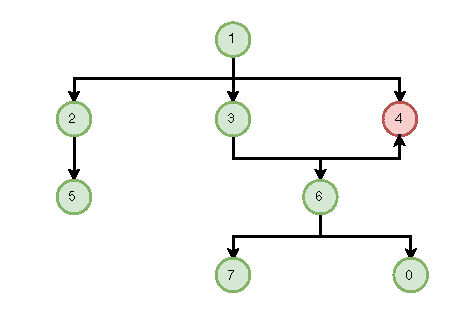
\includegraphics[width=0.4\textwidth]{pdf/tiefensuche8.pdf}
        }      
    \end{center}
    \caption{%
        Tiefensuche im Baum, Knoten aufteigend sortiert in Queue.
     }%

\end{figure}


\begin{figure}[htbp]
     \begin{center}
%
        \subfigure{%
            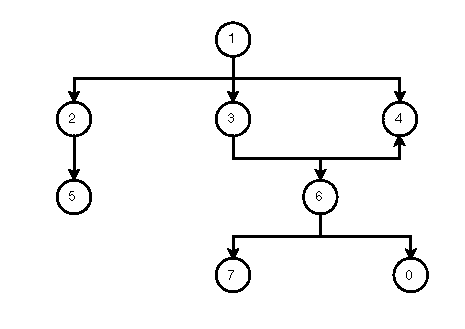
\includegraphics[width=0.4\textwidth]{pdf/tiefensuche0.pdf}
        }%
        \subfigure{%
           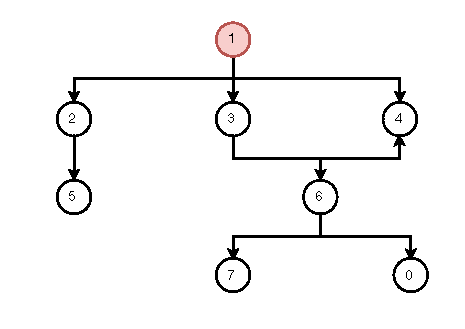
\includegraphics[width=0.4\textwidth]{pdf/tiefensuche1.pdf}
        }\\ %  ------- End of the first row ----------------------%
        \subfigure{%
            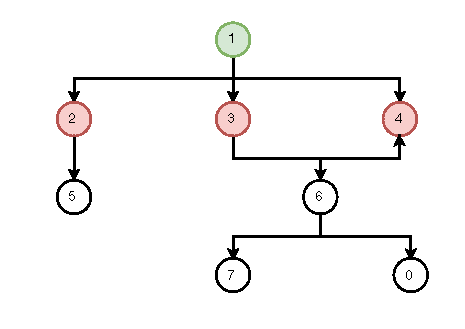
\includegraphics[width=0.4\textwidth]{pdf/tiefensuche2.pdf}
        }%
        \subfigure{%
            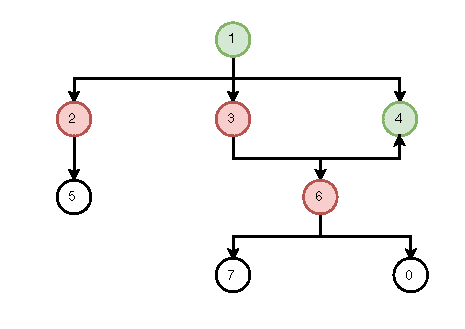
\includegraphics[width=0.4\textwidth]{pdf/tiefensuche3b.pdf}
        }\\%
        
             \subfigure{%
            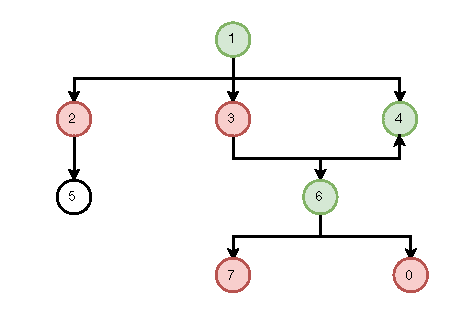
\includegraphics[width=0.4\textwidth]{pdf/tiefensuche4b.pdf}
        }%
        \subfigure{%
            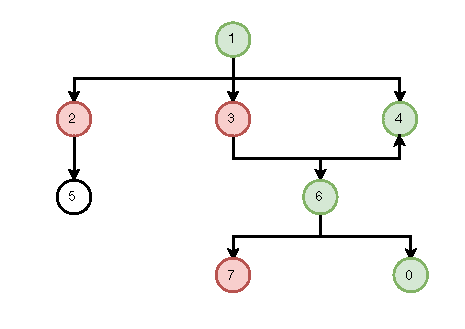
\includegraphics[width=0.4\textwidth]{pdf/tiefensuche5b.pdf}
        }\\     
    \end{center}
    \caption{%
        Tiefensuche im Baum, Knoten absteigend sortiert in Queue.
     }%
\end{figure}

\subsection*{3.1}
\begin{itemize}
\item Breitensuche ist vollständig und bei uniformen Pfadkosten optimal
\begin{itemize}
\item Speicherkomplexität größtes Problem, viele expandierte Knoten
\end{itemize}

\item Tiefensuche ist nicht vollständig und nicht optimal.
\begin{itemize}
\item Deswegen sollte man vermeiden, die Tiefensuche bei Suchproblemen mit großen oder infiniten maximalen Tiefen einzusetzen.
\end{itemize}
\end{itemize}

\end{document}